\documentclass{article}
\usepackage[utf8]{inputenc}
\usepackage[portuges]{babel}
\usepackage{listings}
\usepackage[table]{xcolor}
\usepackage{verbatim}
\usepackage{indentfirst}
\usepackage{hyperref}
%%\setlength{\parindent}{ex}
\usepackage{graphicx}
\usepackage{fancyhdr}
\usepackage{float}

\title{
       \vspace{60px}
       \Huge \textbf{Serviço de transferência rápida e fiável de dados sobre UDP} \\[15px]
       \Large \textbf{Relatório do trabalho prático}
       %%\vspace{100px}
      }
\author{
        \begin{tabular}{c}
            \textbf{Grupo 9} \\[5px]
                Joana Cruz(A76270) \\
                Etienne Costa (A76089) \\
                Hugo Moreira (A43148)
        \end{tabular}
       }
\date{Maio 2019}

\makeatletter         
\def\@maketitle{
    \begin{center}
        \huge \@title \\[4ex]
        \Large \@author \\[5ex] 
        \@date \\[8px]
        \vspace{100px}
        
\includegraphics[scale=0.40]{img/uminho.png} \\
        \vspace{25px} 
        \small Comunicações por Computador \\[3px]
        Mestrado Integrado em Engenharia Informática \\[3px]
        Universidade do Minho \\
    \end{center}}
\makeatother

\begin{document}
\maketitle

\newpage
\section{Introdução}

Este projeto surge no âmbito da Unidade Curricular de Comunicações por Computador e tem como objetivo a implementação de  um serviço de transferência rápida e fiável de dados sobre UDP. Sendo que a comunicação deverá ser feita em unidades de dados que caibam dentro de um datagrama UDP e que sejam enviados e recebidos via Sockets UDP.
Este serviço de transferência é caracterizado por três fases durante uma conexão: início da conexão, transferência de dados e término da conexão.


\section{Especificação do protocolo}

Sendo um protocolo uma convenção que controla e possibilita uma conexão, comunicação e transferência de dados entre dois 
sistemas computacionais, dedicou-se esta secção para explicar o formato das mensagens protocolares bem com as suas interações.

\subsection{Proposta do PDU}

O serviço de transferência rápida e fiável de dados foi implementado, a nível aplicacional, com recurso ao UDP. Sendo assim houve a necessidade de definir um datagrama UDP  que possui as seguintes características :

\begin{itemize}
    \item \textbf{Sequence Number}:Valor utilizado para garantir a entrega ordenada e robustez durante a transferência. 
    \item \textbf{Acknowledge}: Valor utilizado para confirmar a entrega de um segmento.
    \item \textbf{Flag Type}: Valores utilizados para indicar um estado particular da conexão ou para fornecer informação adicional. Portanto,
    podem ser usados para fins de solução de problemas ou para controlar como uma determinada conexão é tratada.\\
    De seguida apresenta-se os possíveis valores para estas flags:
    \begin{enumerate}
    \item \textbf{SYN} - início de uma conexão
    \item \textbf{ACK} - confirmação da recepção de um segmento
    \item \textbf{PSH} - segmento com dados de um ficheiro
    \item \textbf{FIN} - término de uma conexão
    \item \textbf{SYN+ACK} - início de uma conexão
    \item \textbf{JOE DOWN} - download de um ficheiro
    \item \textbf{JOE UP} - upload de um ficheiro
    \item \textbf{EXIT} - objetivo de terminar uma conexão
    \item \textbf{LIST} - listar os ficheiros
    \item \textbf{END TRANSF} - término de uma transferência
    \end{enumerate}
    \item \textbf{Port Number}:Valor que indica a nova porta que o cliente irá responder após ser efetuado o início de uma conexão.
    \item \textbf{Window Size}:Indica em bytes a quantidade de informação que este pode enviar nos próximos pacotes, durante uma conexão.
    \item \textbf{Length Data}: Corresponde em bytes ao tamanho do pacote a ser enviado.
    \item \textbf{CheckSum}: Valor utilizado para verificar a integridade de dados transmititos.
    \item \textbf{File Data}: Corresponde em bytes a informação a ser transferida.
\end{itemize}

\begin{figure}[H]
    \centering
    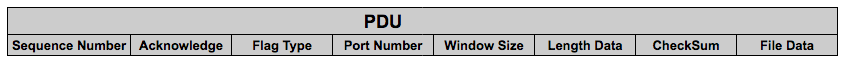
\includegraphics[scale=0.50]{img/pdu.PNG}
    \caption{Protocol Data Unit}
\end{figure}


\subsection{Interação}

O nosso sistema de transferência é caracterizado por três fases distintas durante uma conexão:
\begin{enumerate}
\item \textbf{Início da conexão}
Para o início de uma conexão o nosso sistema foi baseado no 3-Way Handshake do TCP.\\
Sendo que esta conexão procede do seguinte modo:

\begin{table}[h!]
\centering
\begin{tabular}{||c c c c||} 
\hline
\textbf{Início da Conexão} \\ [0.5ex] 
\hline\hline
Host A sends \textbf{SYN}chronize packet to Host B \\ 
Host B receives  \textbf{SYN}  \\
Host B sends  \textbf{SYN}chronize-\textbf{ACK}nowledgment\\
Host A receives  \textbf{SYN-ACK}\\
Host A sends \textbf{ACK}nowledgment \\
Host B receives \textbf{ACK}\\ 
\hline
\end{tabular}
\caption{Início da conexão}
\label{table:1}
\end{table}


\item \textbf{Transferência de Dados}
Para a transferência de dados de forma fiável adoptamos o seguinte mecanismo:
\begin{itemize}
\item O Transmissor vai enviando os segmentos de dados, em que a cada segmento enviado o número do sequência corresponde ao número do segmento
\item O Receptor vai enviando as confirmações dos segmentos recebidos e que não estão corrompidos
\end{itemize}
Uma transferência de dados termina quando o transmissor recebe todos os Acknowledges dos segmentos enviados. Adoptamos um mecanismo de retransmissão seletiva, em
que apenas serão retransmitidos os segmentos de dados do ficheiro que não foram entregues ou que estavam corrompidos. Posteriormente esta explicação
encontra-se mais detalhada.
Agora apresentamos um pequeno exemplo de execução da nossa aplicação de um início de conexão, transferência de um ficheiro(download) e término de uma conexão.
\begin{figure}[H]
\centering
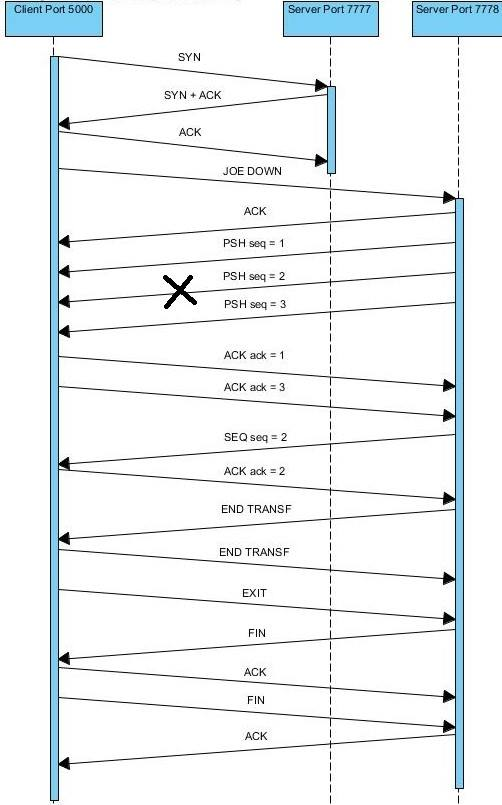
\includegraphics[scale=0.45]{img/diagram.jpg}
\caption{Diagrama temporal de uma transferência}
\end{figure}

\item \textbf{Término da conexão}
Para o término de uma conexão ,o nosso sistema foi baseado no TCP,sendo que este término
é um processo de quatro fases, em que cada sistema computacional é responsável pelo encerramento do seu 
lado da ligação.\\

\begin{table}[h!]
\centering
\begin{tabular}{||c c c c||} 
\hline
\textbf{Término da Conexão} \\ [0.5ex] 
\hline\hline
Host A sends a \textbf{FIN}ished packet to Host B \\ 
Host B receives  \textbf{FIN}ished  \\
Host B sends  \textbf{ACK}nowledgment\\
Host A receives \textbf{ACK}nowledgment\\
Host B sends \textbf{FIN}ished packet to Host A \\
Host A receives \textbf{FIN}ished\\
Host A sends  \textbf{ACK}nowledgment\\
Host B receives \textbf{ACK}nowledgment  \\
\hline
\end{tabular}
\caption{Término da conexão}
\label{table:2}
\end{table}
\end{enumerate}


\newpage

\section{Implementação}

\subsection{Arquitetura da solução}
A arquitetura da nossa solução difere um pouco da pedida no enunciado, dado que estruturámos o nosso problema como sendo Servidor e Cliente.
O Servidor encontra-se sempre à escuta na porta 7777 de pedidos de conexão de clientes. Quando um cliente se pretende conectar, o servidor
terá que aceitar a conexão pedida, e aí dá-se o mecanismo de início de conexão descrito anteriormente. Após este mecanismo, o Servidor
abre um novo Socket que será responsável de satisfazer os pedidos do cliente, podendo aceitar pedidos de outros clientes pois a porta 7777 
assim continua à escuta de outros pedidos de conexão. O cliente após estar conectado poderá listar os ficheiros disponíveis no Servidor, fazer download
ou upload de um ficheiro, e terminar uma conexão. 

\subsection{Estrutura de dados}
Para a implementação destes conceitos, foi utilizada a linguagem de programação orientada a objectos \emph{Java}, e foram definidas as seguintes classes.\\
\par \textbf{Classes relacionadas com o Cliente:}
\begin{itemize}
\item \textbf{ClientMain} - Classe main do cliente
\item \textbf{ClientAgentUDP} - Classe principal do cliente que contém métodos de início e término de conexão, assim como download e upload de ficheiros.\\
\\
\textbf{Classes relacionadas com o Servidor:}
\item \textbf{ServerMain} - Classe main do Servidor
\item \textbf{ServerAgentUDP} - Thread responsável por estar sempre à escuta de pedidos de conexões de clientes distintos
\item \textbf{ClientHandler} - Thread responsável por estar à escuta de diversos pedidos de um cliente\\
\\
\textbf{Classes comuns ao Servidor e Cliente:}
\item \textbf{PDU} - classe que corresponde à estrutura de PDU que irá ser enviada nos Sockets UDP
\item \textbf{Resources} - classe com os recursos de uma conexão, contém variáveis como o socket, a porta de envio, o endereço IP e todos os métodos associados ao envio e recepção de um segmento
\item \textbf{FileSender} - Thread responsável por mandar um ficheiro
\item \textbf{AckReceiver} - Thread responsável por receber os ACKs 
\item \textbf{FileReceiver} - Thread responsável por receber segementos correspondentes a um ficheiro
\item \textbf{AckSender} - Thread responsável por mandar ACKs dos segmentos do ficheiro que já recebeu
\end{itemize}

\subsection{Modo de funcionamento}
Como já foi referido anteriormente o Servidor encontra-se sempre à escuta na porta 7777. Após efetuar o início de uma conexão,
abre um novo Socket, e a Thread ClientHandler estará sempre à escuta de pedidos desse cliente. Conforme o pedido efetuado o procedimento vai ser
diferente. Aqui iremos apresentar o procedimento caso o cliente peça um download de um ficheiro. Então quando o cliente pede um download
4 novas threads irão começar a trabalhar, duas no lado do Servidor e duas no Cliente. Cada par trabalha em conjunto, como um Receptor e um Transmissor.\\ \\
\textbf{No lado do Servidor:} \\
Então no Servidor que neste caso será o Transmissor, a Thread fileSender estará responsável por enviar PDUs com a informação do ficheiro no
máximo 1024 bytes de cada vez, enquanto a thread AckReceiver estrá responsável por estar à escuta, esperando por segmentos que sejam
Acknowledges recebidos pelo Cliente. Estas 2 Threads partilham uma estrutura de dados(Thread safe), sendo que sempre que a FileSender envia
um segmento com o respetivo número de sequência adiciona ao HashMap(o número de sequência e o respetivo PDU), ao mesmo tempo que a AckReceiver irá
retirar desse HashMap sempre que recebe um Acknowledge. Após a FileSender ter enviado todos os segmentos do ficheiro, irá apenas retransmitir
os segmentos dos quais não recebeu ACKs. Quando esta estrutura estiver vazia quer dizer que todos os segmentos foram entregues ao Receptor, 
e será enviado um PDU com a informação que a transferência foi efetuada com sucesso.\\ \\
\textbf{No lado do Cliente:} \\
No Cliente estará à escuta(esperando por receber segmentos) a Thread FileReceiver, e responsável por enviar PDUs de confirmação será a AckSender.
O mecanismo é o mesmo utilizado no Servidor, ambas as Threads partilham de uma estrutura, e a FileReceiver vai adicionando à estrutura,
enquanto a AckSender retira da estrutura os ACKs que enviou. Quando a FileReceiver receber um PDU com a flag END TRANSF, saberá que a
transferência foi efetuada com sucesso, e enviará uma confirmação.\\ \\
\textbf{Observações:}\\
\begin{itemize}
\item Para controle de erros: A FileSender calcula sempre o checksum antes de ser enviado o segmento, incluindo esse valor no PDU enviado.
Enquando que a FileReceiver, quando recebe o segmento faz esse mesmo exato cálculo, e verifica se o pacote não está corrompido, e apenas
adiciona à estrutura partilhada se o pacote não estiver corrompido. Para o cálculo do checksum usou-se uma classe já pré-definida pelo Java e a sua respetiva API - CRC32.
\item Para controlo de fluxo: Para que o emissor não extravase o buffer do emissor enviámos 10 segmentos de cada vez, adormecendo a FileSender
durante milisegundos, e reenviando o resto dos segmentos outra vez.
\end{itemize}
De seguida apresentamos uma imagem ilustrativa do processo descrito.
\begin{figure}[H]
\centering
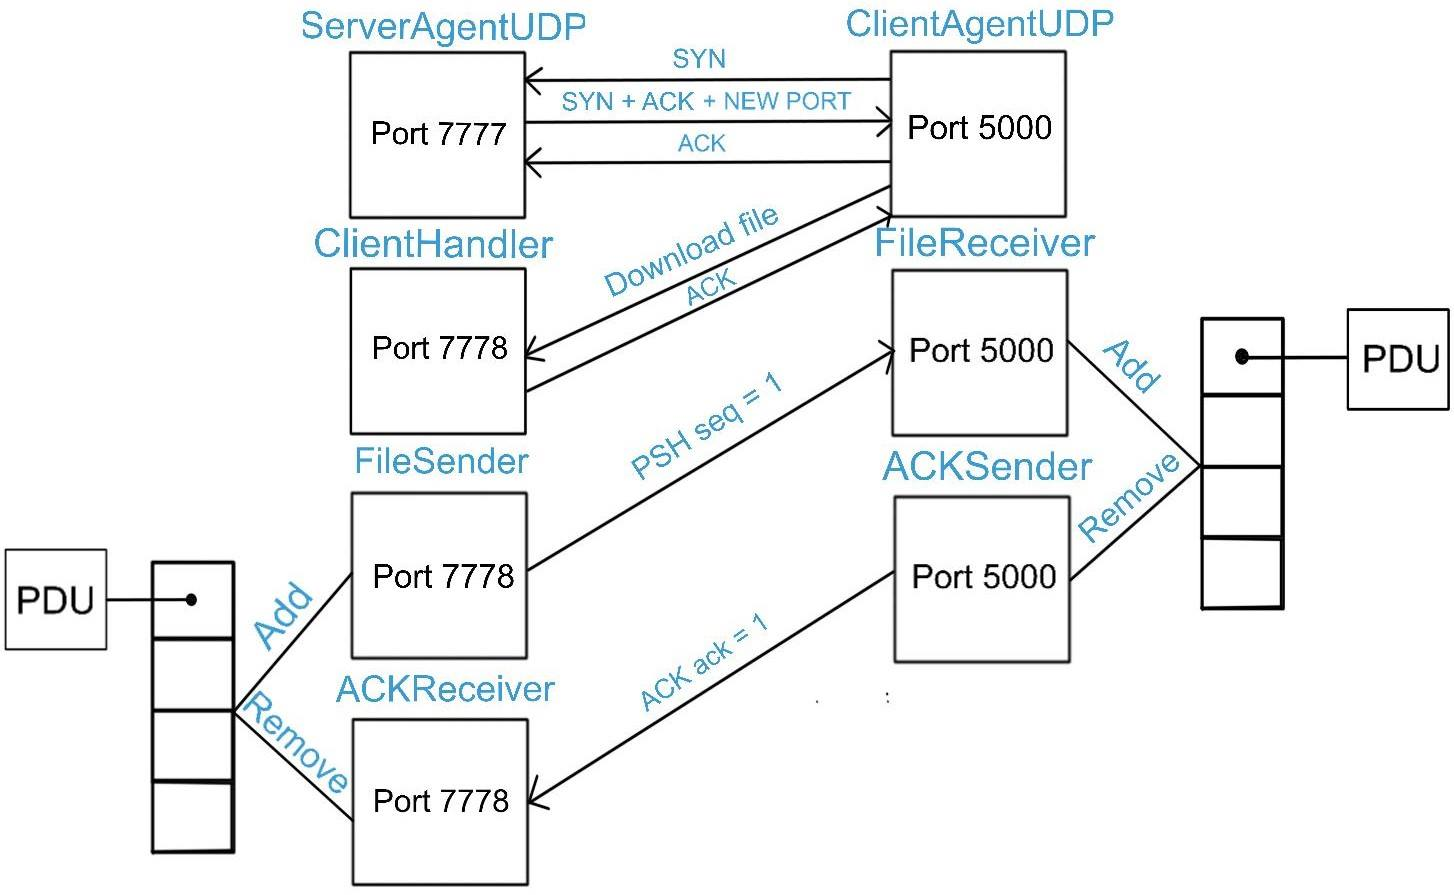
\includegraphics[scale=0.25]{img/imagem.jpg}
\caption{Arquitetura da solução implementada}
\end{figure}
Caso o pedido fosse um upload do ficheiro, o mecanismo seria o inverso, dado que o Cliente funcionava como Transmissor e o Servidor como Receptor.
\subsection{Métodos}
De modo a não tornar esta leitura exaustiva , decidiu-se simplesmente apresentar os métodos mais relevantes
e procurar explicar o impacto que cada um tem na implementação do nosso serviço. \\
Na classe PDU, estes métodos foram necessários para troca de segmentos UDP:
\begin{enumerate}
\item \textbf{ByteToPDU} - converte um array de bytes num objeto PDU
\item \textbf{PDUToByte} - converte um objeto PDU num array de bytes
\end{enumerate}
Na classe Resources:
\begin{enumerate}
\item \textbf{receive} - Método que recebe um DatagramPacket, e converte os bytes recebidos num PDU
\item \textbf{receive(int timeout)} - Igual ao método anterior, mas agora com um timeout pré-estabelecido para receber um segmento
\item \textbf{send(PDU packet)} - Método que converte um PDU num array de bytes, e envia um DatagramPacket
\item \textbf{sendAndExpect(PDU packet, int timeout, int attemps)} - Método que envia um PDU, e caso não receba um segmento de volta durante um perído de tempo, tenta enviar o segmento X vezes até receber um segmento de volta.
\end{enumerate}
Na classe ClientAgentUDP:
\begin{enumerate}
\item \textbf{connect} - Método de conexão do cliente
\item \textbf{disconnect} -  Método de término de conexão do cliente
\item \textbf{downloadFile} - Método em que o cliente funciona como receptor
\item \textbf{uploadFile} - Método em que o cliente funciona como transmissor
\end{enumerate}

Consíderamos o método sendAndExpect o mais importante, pois dado que o UDP não garante a recepção de segmentos, também teríamos que considerar
que poderiam haver perdas de pacotes no ínicio de uma conexão, num pedido de um cliente, no término de uma conexão. O nosso serviço
está preparado para perda de qualquer segmento, e não apenas durante uma transferência. 

\subsection{Bibliotecas de suporte}

Sendo java uma linguagem de programação bastante versátil foi possível importar todas as bibliotecas que permitissem a realização 
deste projecto,sendo elas as seguintes:

\begin{itemize}
\item{java.net.InetAddress;}
\item{java.util.concurrent.ConcurrentHashMap;}
\item{java.util.concurrent.atomic.AtomicBoolean;}
\item{java.util.Scanner;}
\item{java.net.UnknownHostException;}
\item{java.net.SocketException;}
\item{java.io.IOException;}
\item{java.net.SocketTimeoutException;}
\item{java.io.FileOutputStream;}
\item{java.io.FileInputStream;}
\item{java.util.Arrays;}
\item{java.util.zip.CRC32;}
\item{java.nio.ByteBuffer;}
\item{java.net.DatagramPacket;}
\item{java.net.DatagramSocket;}
\end{itemize}
\subsection{Comandos}
O cliente na nossa aplicação poderá utilizar os seguintes comandos:
\begin{itemize}
\item list - lista os ficheiros disponíveis no Servidor
\item download $<$fileLocalName$>$ ou download $<$fileLocalName$>$ $<$fileRemoteName$>$ - download de um ficheiro, com possibilidade de escolha de um nome remoto
\item upload $<$fileLocalName$>$  - upload de um ficheiro para o Servidor
\item help - menu de ajuda para visualizar os comandos disponíveis
\item exit - término de uma conexão, e consequentemente fecho do socket
\end{itemize}
\newpage

\newpage
\section{Testes e Resultados}
Nesta secção apresentamos alguns testes efetuados no core que achamos relevantes. Primeiramente o início de conexão de 2 Clientes, sendo
que um encontra-se numa ligação segura, e outro com perda e duplicação de pacotes.
\begin{figure}[H]
\centering
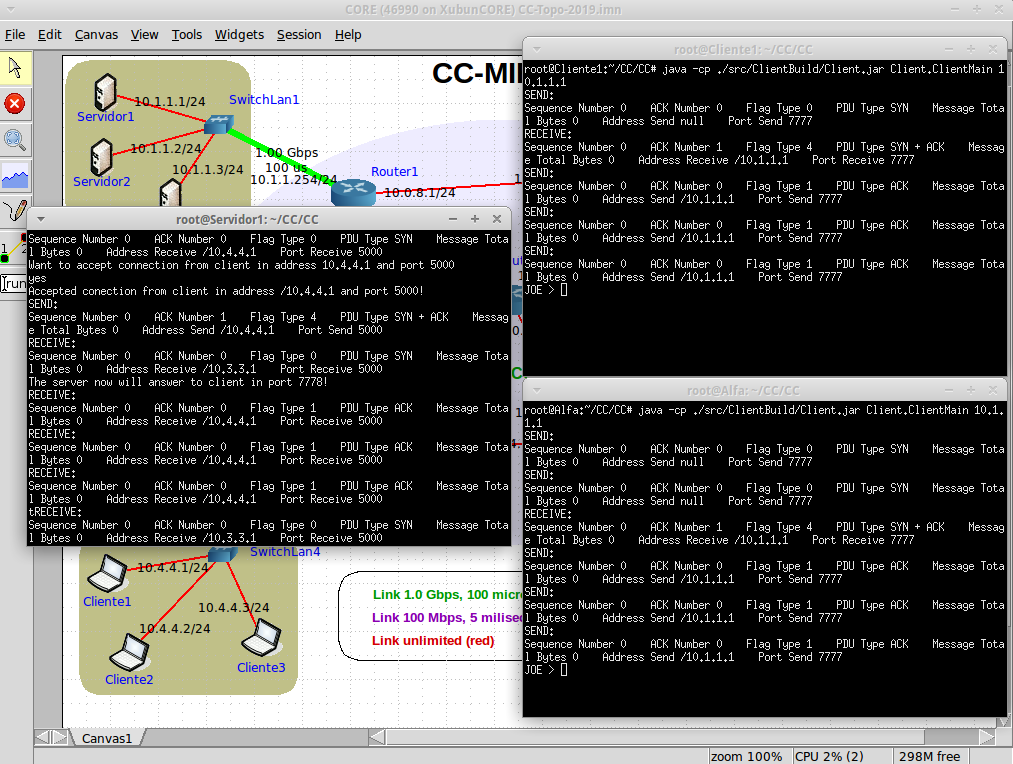
\includegraphics[scale=0.4]{img/connection.png}
\caption{Conexão de clientes}
\end{figure}
Posteriormente apresentamos um dos clientes a pedir a lista de ficheiros disponíveis no Servidor.
\begin{figure}[H]
\centering
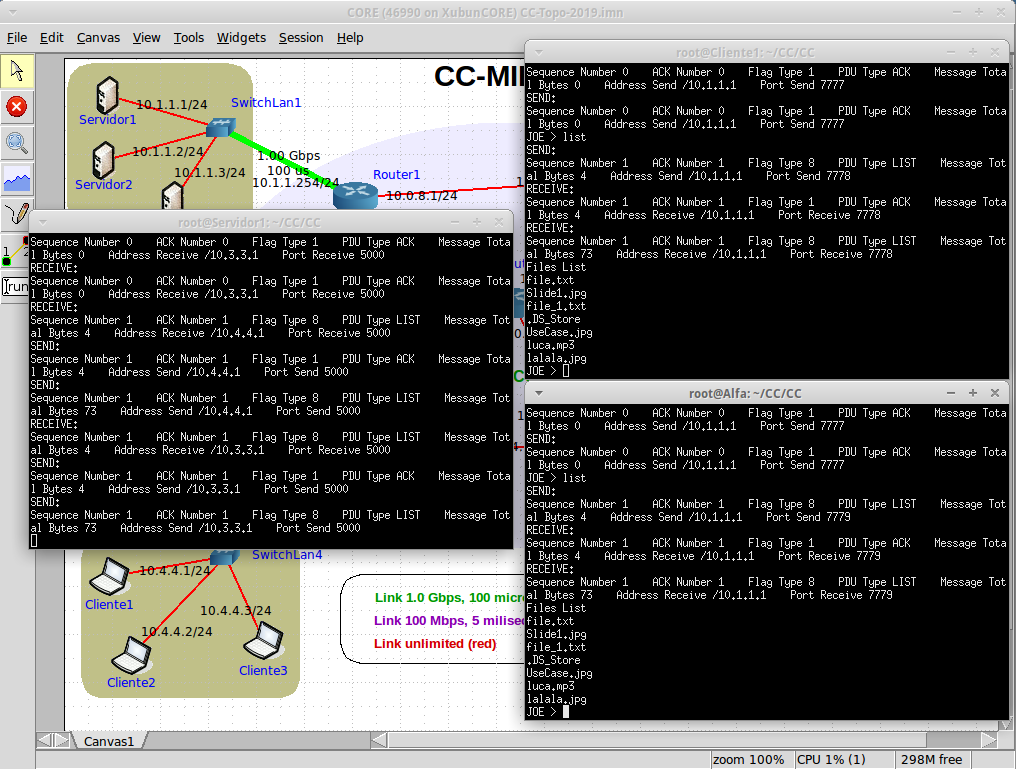
\includegraphics[scale=0.4]{img/list.png}
\caption{Pedido da lista de ficheiros}
\end{figure}
Por último, a execução do download de um ficheiro MP3 pelos 2 clientes no mesmo instante.
\begin{figure}[H]
\centering
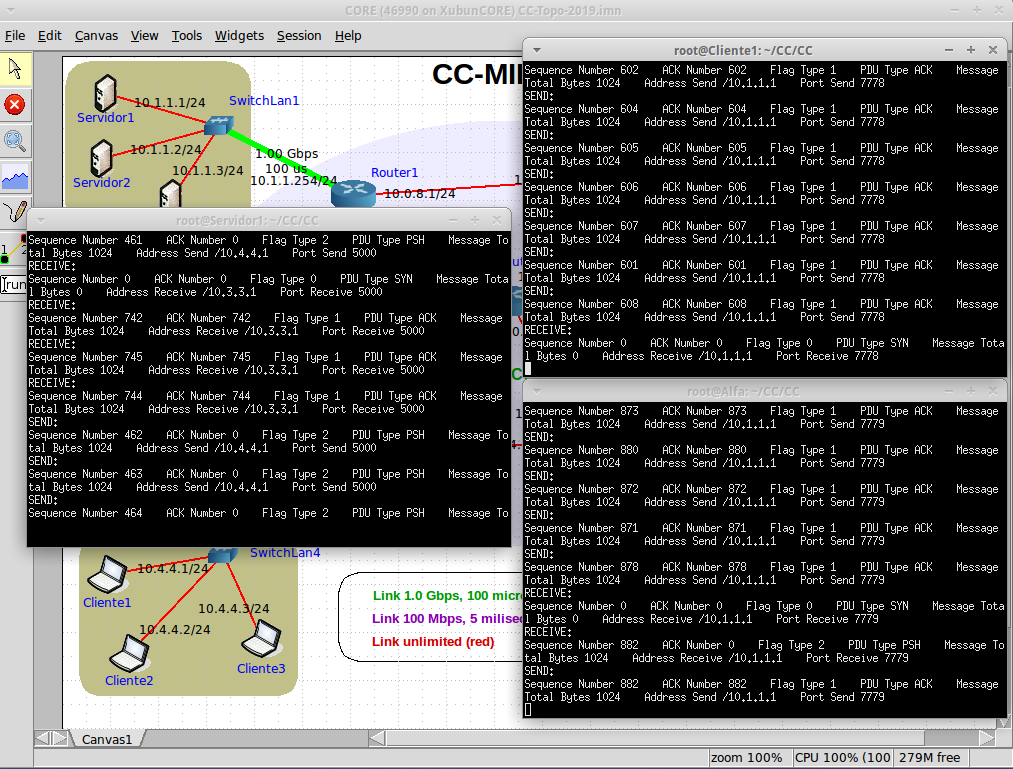
\includegraphics[scale=0.4]{img/download.png}
\caption{Pedidos de transferência de ficheiro}
\end{figure}
Para uma fase de desenvolvimento e de testes decidimos demostrar os prints de todos os segmentos enviados e recebidos tanto pelo Servidor e
pelos Clientes que funciona como a nossa Tabela de Estado. Sendo que estes prints apresentam sempre a informação do número de sequência,
número de ACK, tipo de PDU, tamanho dos dados transferidos, porta e o endereço IP.
\newpage
\section{Conclusões e trabalho futuro}
Inicialmente tivemos algumas dificuldades na estruturação do trabalho, nomeadamente qual o mecanismo que adoptaríamos para que a recepção de qualquer segmento
enviado fosse de forma fiável, assim como efetuar as retransmissões, que após uma análise detalhada
do problema foram ultrapassadas. Implementámos todas as funcionalidades obrigatórias propostas, dado que a solução de transferência
de um ficheiro não foi a ideal dado o espaço em memória utilizado pelas estruturas partilhadas pelas Threads. Por outro lado, consíderamos
a nossa solução eficiente pois em qualquer transferência, tanto no Transmissor como no Receptor, temos uma Thread responsável 
pela recepção de segmentos e outra pelo envio. Quanto às funcionalidades adicionais apenas as múltiplas conexões em simultâneo foi 
implementada, 
sendo assim numa perspectiva de trabalho futuro serão implementas mais funcionalidades de modo a tornar o sistema mais complexo. 
\end{document}
